\documentclass[12pt]{llncs}
\usepackage{tikz}
\usepackage{float}
\usepackage{amsmath}
\usepackage{graphicx}
\usepackage{subcaption}

\usetikzlibrary{calc}
\usepackage[
	backend=bibtex,
	style=numeric,
	sorting=none]{biblatex}
\addbibresource{references.bib}

\title{Modeling SARS-CoV-2 pandemic in NetLogo}
\author{Lorenzo Vainigli \\
lorenzo.vainigli@studio.unibo.it \\
matr. 0000842756}
\institute{Course of Complex Systems and Network Science \\
Laurea Magistrale in Informatica \\
University of Bologna \\
A.Y. 2020-2021}
\date{\today}

\pagestyle{plain}

\begin{document}
{\def\addcontentsline#1#2#3{}\maketitle}

\begin{abstract}
The SARS-CoV-2 outbreak has forced the world population to face a new disease for which there was not a vaccine and governments had to use some alternative actions to limit the virus spreading. Predicting the impact of an action on the population is very important before making it effective and we need mathematical models to do that. This paper shows the implementation of a virus outbreak in NetLogo and it provides actions to limit the spreading: quarantine, isolation, social distance and lockdown. Every action can be enable or disable and it has parameters that can be set. A study on how these actions can help to fight and slow down the virus propagation is described and results that prove the effectiveness of these containment measures are shown.
\end{abstract}

\begingroup
\let\clearpage\relax
\renewcommand{\contentsname}{}
\setcounter{tocdepth}{2}
\tableofcontents
\endgroup

\section{Introduction}
This paper describes the process of building and studying a network model that simulates the outbreak of the new SARS-CoV-2 virus using NetLogo. In addition, the model provides methods to control the spreading. To achieve this challenge, we must consider a situation in which we have a crowd of people, each of which have contacts with others and where there are some infected individuals that cause the spreading of the infection. Also some kind of quarantine and isolations are needed for who become infected. Finally we need some population-size actions like social distancing and lockdown, beacause these are the most used and effective actions that have been used by governments to reduce the impact of the virus on the population.\\
Our model provides all the features mentioned above with different paramaters that can be changed in order to set the strenghtness of the containment measures.\\
Once we have found a setting of parameters that causes, more or less, the same effects on the population as the real virus did, we focus our experiments in studying the effects of the containment measures on the virus impact on the population. Results we got clearly show that these actions are effective and can save lives.

\section{Preliminaries}
The literature about virus diffusion is very rich because 2020 has been a year in which the researchers need to discover everything about the new SARS-CoV-2 virus and the COVID-19 disease \cite{singhal}. Models to represent situations like this or other diseases like flu were developed by Brauer et al. \cite{brauer}; one of these, the \textit{SEIQRJ} model, is suitable to study the SARS-CoV-2 pandemic. An article from Giordano et al. explains how to model the intervetions in the population to fight the COVID-19 outbreak \cite{giordano}, but it's too complex for the purposes of this project. The Netlogo \cite{netlogo} models library offers an implementation of the \textit{SIR} model \cite{netlogo-virus}: it's very simple and it's a good point to start the implementation of our model.\\ 
In this project, the modelling phase started from the \textit{SEIQJR} model shown by by Brauer et al. and the implementation phase started from the Virus model from the NetLogo library.

\section{Modeling}
In this section we will explain the process of building the model that will be implemented to realize this project.\\
We start from the scheme of the \textit{SEIQJS} model, explaining why this model is the one we need for our purpose and then we conclude this section explaining how to model contact tracing, social-distance and lockdown.

\subsection{The SEIQJS model}
Before showing the diagram of the model that we will use, let's see how it was constructed.\\
The \textit{SIS} model is the simplest model in which there is a class of susceptible people ($S$) that, if one get the infection, goes to the infected class ($I$). Then, when infected people get recovered they returned to the susceptible class.
As we know, SARS-CoV-2 infection leads an incubation period during which the infected person don't have symptoms but can transmit the infection to other people. We introduce an exposed class $E$ in which we put people that had have a contact with infected people and may be infected in an asymptomatic status.
Due to the unavailability of a vaccine, to fight SARS-CoV-2 infected people are quarantined or isolated (or, also, hospitalized). As suggested from the \textit{SEIQJR} model, two classes were added: $Q$ is the class of quarantined people, i.e. the exposed people belong to the class $E$; $J$ is the class for isolate infected people of class $I$. So basically $Q$ is for $E$ what $J$ is for $I$, with the only difference that there is a flow from $Q$ to $J$ but not vice versa.\\
People isolated (i.e. belong to class $J$) can recover as people belong to class $I$. Finally, a class $D$ is added where dead people go.

\paragraph{\textbf{No immunity provided}}
Beacuse of the unknown properties of immunity from SARS-CoV-2, we can assume that the S class and R class coincide, creating a cycle that causes the comeback of the recoverd individuals in the susceptible class, if they don't die.
\\\\
\textit{Classes}
\begin{multicols}{3}
\begin{itemize}
\item $S$ = Susceptible
\item $E$ = Exposed
\item $I$ = Infected
\item $Q$ = Quarantined
\item $J$ = Isolated
\item $D$ = Dead
\end{itemize}
\end{multicols}

\paragraph{New variables}
\begin{itemize}
\item $a$ = infection rate;
\item $\varepsilon_E$ = probability that a person exposed (in $E$) transmit the infection, exposed-transmission-factor;
\item $\varepsilon_Q$ = probability that a person quarantined (in $Q$) make a contact, quarantined-contact-factor;
\item $\varepsilon_J$ = probability that a person isolated (in $J$) transmit the infection, isolation-transmission-factor;
\item $k_E$ = probability that exposed people become infective;
\item $k_Q$ = probability that quarantined people are isolated;
\item $c_Q$ = percentage of exposed people that are quarantined at each time step;
\item $c_J$ = percentage of infected people that are isolated at each time step;
\item $b_I$ = probability that an infected person left the infected class;
\item $b_J$ = probability that an isolated person left the isolated class;
\item $r_I$ = probability that an infected person get recovered, otherwise he die;
\item $r_J$ = probability that an isolated person get recovered, otherwise he die.
\end{itemize}
The diagram of the model is shown in fig. \ref{fig:model} and the equations are shown in eq. \ref{eq:model}.

\begin{figure}
	\centering
    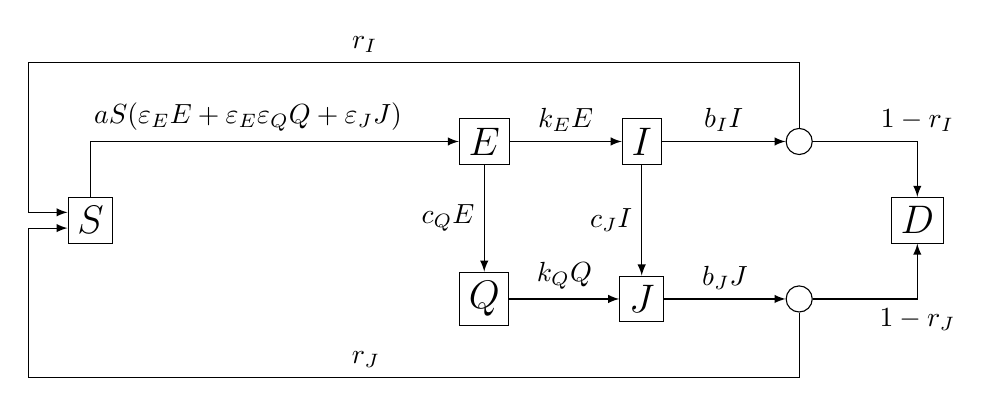
\begin{tikzpicture}
    \node[draw] at (0,0) (S) {\Large $S$};
    \node[draw] at (5,1) (E) {\Large $E$};
    \node[draw] at (5,-1) (Q) {\Large $Q$};
    \node[draw] at (7,1) (I) {\Large $I$};
    \node[draw] at (7,-1) (J) {\Large $J$};
    \node[draw] at (10.5,0) (D) {\Large $D$};
    \node[draw,circle,minimum size=3pt] at (9,1) (Ib) {};
    \node[draw,circle,minimum size=3pt] at (9,-1) (Jb) {};
    \draw[draw, -latex] (S.north) |- (E.west) node [midway,xshift=2cm,above] {$aS(\varepsilon_EE + \varepsilon_E\varepsilon_QQ + \varepsilon_JJ)$};
    \draw[draw, -latex] (E.south) -- (Q.north) node [midway,left] {$c_QE$};
    \draw[draw, -latex] (E.east) -- (I.west) node [midway,above] {$k_EE$};
    \draw[draw, -latex] (I.south) -- (J.north) node [midway,left] {$c_JI$};
    \draw[draw, -latex] (Q.east) -- (J.west) node [midway,above] {$k_QQ$};
    \draw[draw, -latex] (I.east) -- (Ib.west) node [midway,above] {$b_II$};
    \draw[draw, -latex] (J.east) -- (Jb.west) node [midway,above] {$b_JJ$};
    \draw[draw, -latex] (Ib.north) |- ($(I.east)+(0.5,1)$) -- ($(S.west)+(-0.5,2)$) node [midway,above] {$r_I$} |- ($(S.west)+(0,0.1)$);
    \draw[draw, -latex] (Jb.south) |- ($(J.east)+(0.5,-1)$) -- ($(S.west)-(0.5,2)$) node [midway,above] {$r_J$} |- ($(S.west)-(0,0.1)$);
    \draw[draw, -latex] (Ib.east) -| (D.north) node [midway,above] {$1-r_I$};
    \draw[draw, -latex] (Jb.east) -| (D.south) node [midway,below] {$1-r_J$};
    \end{tikzpicture}
    \caption{Diagram of the SEIQJS model}
    \label{fig:model}
\end{figure}

\begin{equation}
\begin{aligned}
&\frac{dS}{dt} = -aS(\varepsilon_EE + \varepsilon_E\varepsilon_QQ + \varepsilon_JJ) + b_Ir_II + b_Jr_JJ\\
&\frac{dE}{dt} = aS(\varepsilon_EE + \varepsilon_E\varepsilon_QQ + \varepsilon_JJ) - (k_E + c_Q)E\\
&\frac{dQ}{dt} = c_QE - k_QQ\\
&\frac{dI}{dt} = k_EE - (b_I + c_J)I\\
&\frac{dJ}{dt} = k_QQ + c_JI - b_JJ\\
&\frac{dD}{dt} = b_I(1-r_I)I + b_J(1-r_J)J\\
\end{aligned}
\label{eq:model}
\end{equation}

\subsection{Action to limit the epidemic spread}
In a context of epidemic spread some actions can carried out to protect the health of the population. Basically, because of the virus infection is transmitted during contacts person-to-person, these contacts must be reduced. Putting the exposed or infected people in quarantine or isolation is the best thing to do, but also methods of social distancing or mobility restrictions can be used. \\
In this project we implemented quarantine, isolation, social distance and lockdown.

\subsection{Contact tracing and evaluation method}
As we know that SARS-CoV-2 infection leads to an asymptomatic status, a contact tracing technique can be used to find people who can transmit the virus before that they become symptomatic. In this model we built a contact tracing technique not properly to find potential infected individuals, but to evaluate the amount of contacts in each simulation to have an indicator of the power of the virus spreading. What is important to notice is that the more contacts we have between people, the more powerfull the outbreak will be and thus the harder will be to control it.

\section{Implementation}
In this section we describe the way we implemented the concepts shown in the previous section.

\subsection{The base model}
The Virus model from the NetLogo library \cite{netlogo-virus} is the point from which we started the development of our model. The Virus model is an implementation of the \textit{SIR} model, with some peculiarities:
\begin{enumerate}
\item people can reproduce;
\item people can recover from the infection but they can also die;
\item recovered individuals have a phase of immunity before they come back to the susceptible class.
\end{enumerate}
As previously stated, we conclude that immunity is not a characteristic that we want to have in our final model, so we remove the class of immune people, but we keep the behavior of reproduction and death.

\subsection{Parameters}
The parameters of the model are the ones described for the \textit{SEIQJS} model, divided into \textit{fixed parameters}, i.e. the ones that are specific to the virus and that we cannot change, and the \textit{control parameters}, which can be tuned in order to study attempts to manage the epidemic.

\paragraph{Fixed parameters}
\begin{itemize}
\item \texttt{infection-rate} ($a$);
\item \texttt{exposed-transmission-factor} ($\varepsilon_E$);
\item \texttt{exposed-to-infected-rate} ($k_E$);
\item \texttt{quarantined-to-isolated-rate} ($k_Q$);
\item \texttt{infected-leave-rate} ($b_I$);
\item \texttt{isolated-leave-rate} ($b_J$);
\item \texttt{infected-chance-recover} ($r_I$);
\item \texttt{isolated-chance-recover} ($r_J$).
\end{itemize}

\paragraph{Control parameters}
\begin{itemize}
\item \texttt{quarantine-perfection} ($\varepsilon_Q$);
\item \texttt{isolation-perfection} ($\varepsilon_J$);
\item \texttt{quarantines-per-day-rate} ($c_Q$);
\item \texttt{isolations-per-day-rate} ($c_J$);
\item \texttt{social-distance-perfection};
\item \texttt{lockdown-strictness}.
\end{itemize}
The last two parameters, even if they are not part of the \textit{SEIQJS} model, are used to manage the epidemic.\\
Experiments with this model are made by trying different values for control parameters, while fixed parameters remain unchanged.

\subsection{Class representation}
The \textit{SEIS}, \textit{SEIQJR} and other similar diagrams have a fundamental constraint: at each time step, a person of the population (i.e. an agent) must belong to one and only one class. This is done by simply add five properities to the agent: one of each indicates a different class, so at each time step, one of these property must be \texttt{true} and the others \texttt{false}. This fact does not apply to the class of dead people, beacuse it is a class without exit: if a person dies, the agent is killed and the deadth counter increased by one.

\subsection{Class transitions methods}
To make possible that a person change class a series of methods were implemented. All of them share a similar structure:
\begin{enumerate}
\item check if the candidate that is going to go to the class actually belongs to a class from which a flow from the two classes is defined (If $p$ want to go from $A$ to $B$ a transition $A \rightarrow B$ must be defined). Throw an error if is not possibile;
\item put to \texttt{false} the properties of the person that could hold the value \texttt{true};
\item put to \texttt{true} the property that indicates the new class.
\end{enumerate}
These methods are \texttt{get-exposed}, \texttt{get-quarantined}, \texttt{get-infected}, \texttt{get-isolated} and \texttt{get-recovered}.

\subsection{Core procedures: setup and go}
Every NetLogo model is based on these two procedures:
\begin{itemize}
\item \texttt{setup} is the function that provides the initialization of the model before every simulation;
\item \texttt{go} is the function that will be executed every time step (tick).
\end{itemize}

\paragraph{The procedure \texttt{setup}} creates the turtles that represent the population and initialize their properties: every turtle is putted in the susceptible class. To create the beginning of virus spreading, after these actions some of the created turtles are picked at random and moved to the exposed class and to the infected class.\\

To understand the explaination of the following procedure \texttt{go} we need to underline first a design choice: we decided to let that some actions occurs more often that others, below I explain which they are and why. To implement this behaviour we used a new variable that counts the days elapsed from the beginning of the simulation, every time \texttt{ticks} is a multiplier of \texttt{ticks-per-days}, days counter advances by one.\\
Why this design choice? Every tick people make a single move, so it's strange that the mechanism of quarantine and isolate people occurs with the same frequency. Distinction between \texttt{ticks} and \texttt{days} makes the simulation more realistic.

\paragraph{The procedure \texttt{go}} calls various other procedures that carried on the simulation and the behaviour of the model, but they are divided into two groups:
\begin{itemize}
\item \textit{once-per-tick} procedures that are called every time the \texttt{go} procedure is called, so every tick
\begin{itemize}
\item people motion in the enviroment, 
\item people transition to exposed class due to a contact with an infected person,
\item contract tracing update;
\end{itemize}
\item \textit{once-per-day} procedures that are called every time the day counter advanced:
\begin{itemize}
\item every class transition except the one from susceptible to exposed, that, as we stated previously, happens for every tick.
\end{itemize}
\end{itemize}

\subsection{Virus propagation}
The infection spreading of the virus in the population is implemented in the function \texttt{infect} that looks a little bit complicated but, essentialy, uses the parameters of the model to call, in a proper way, the procedure \texttt{get\_exposed}. It's the only procedure that makes call to \texttt{get\_exposed}. Take a look to the comments in the code of the model to know more.

\subsection{Contact tracing}
Contact tracing is implemented using the construct \texttt{link} of NetLogo. At each time step, the program asks to each person to create a link with other people that share, in that moment, the same patch. Basically is the same way that the virus spreads and it has a sense beacuse the aim of contact tracing is to track the propagation of the virus. The result is a graph connecting people to each others.

\subsection{Social distance and lockdown}
Two methods were implemented to control people movement in order to reduce contacts between them: social distance and lockdown
\paragraph{Social distance} can be enabled or disabled in this model and uses an auxiliry parameter called \texttt{social-distance-perfection}. If social distance is disabled, people are free to move everywhere, while if it's enabled people avoid to move to a patch that is already occupied by others with an error probability of determined by $1 - \textrm{\texttt{social-distance-perfection}}$.
\paragraph{Lockdown} is implemented taking into account a value that defines the probability that a person will move or not. \\
If the variable \texttt{lockdown-strinctness} is set to zero, people are completely free to move, while if the value increases, people will make a move with less probability. If a person doesn't move, it remain in the same patch where it was previously.\\ \\
Take a look to the procedure \texttt{move} to find the code about these control measures.

\subsection{Evaluation}
In this model we considered to evaluate every situation analyzing the graph generated by the contact tracing method. The more connected is the graph, the more powerful is the virus spreading and so, in a real situation, the more stressed the health system will be.\\
We use the definition of \textit{degree centrality} to have a clear indicator of the connections that each person creates during simulation. Beacause of degree centrality is a node-based measure, we used the average of all the degree centralities to get a value to evaluate the entire graph. An auxiliary indicator of standard deviation for this average is provided. \\
If a control action on the population reduces the value of \textit{average degree centrality}, it means that the action is effective.

\section{Results}\label{results}
In this section we describe the results obtained making simulations with this model. Differences between simulations are about watch how the simulation evolves with different actions.\\
The size of the population at the beginning of the simulations is fixed at 150 and the duration of the simulations is 365 days.

\subsection{Virus diffusion without actions}
The first thing to do to have an idea of what happens is to watch the behavior of the model if nothing action to fight the virus is taken. As we can see in fig. \ref{fig:noactions-a} the lethality of the virus makes an unacceptable impact on the population, reducing it to few individuals. The reduction of the \textit{average degree centrality} (fig. \ref{fig:noactions-b}) is only due to the decrease of the population.

\begin{figure}
	\begin{subfigure}{\textwidth}
	\centering
		\includegraphics[width=0.9\textwidth]{results/no_actions_population.png}
		\caption{Evolution of the population divided by class.} \label{fig:noactions-a}
	\end{subfigure}
	\begin{subfigure}{\textwidth}
	\centering
		\includegraphics[width=0.9\textwidth]{results/no_actions_degree_centrality.png}
		\caption{Evolution of the values of degree centrality.} \label{fig:noactions-b}
	\end{subfigure}
	\caption{Result of the simulations without actions to control the diffusion of the virus. Population has been reduced by \textbf{96\%} and \textbf{147} people were dead.}
\end{figure}

\subsection{Using only quarantine and isolation}
Let's see how using quarantine and isolation will change the virus diffusion and thus the results after a simulation. These measure prevent the people to move but not to making contacts, even if with a lower probability. We can see in fig. \ref{fig:quar-isol-a} the huge impact that these measures make in the simulation, saving the 29,3\% of the population with respect to the previous situation. In fig. \ref{fig:noactions-b} we can se a visible reduction of contacts between people. Simulation is carried out with these settings:
\begin{itemize}
\item \texttt{quarantine-perfection} = 70
\item \texttt{quarantines-per-day-rate} = 10
\item \texttt{isolation-perfection} = 90
\item \texttt{isolations-per-day-rate} = 10
\end{itemize}

\begin{figure}
	\begin{subfigure}{\textwidth}
	\centering
	\resizebox{0.9\textwidth}{!}{
		\begin{tikzpicture}
	\node[inner sep=0pt] at (0,0) {\includegraphics[width=\textwidth]{results/quarantine_isolation_population.png}};
	\node[text width=4cm,align=left] (label) at (0,1) {Activation of quarantine and isolation};
	\draw [->] (label.west) -| (-3.1,-1);
    \end{tikzpicture}
    }
		\caption{Evolution of the population divided by class.} \label{fig:quar-isol-a}
	\end{subfigure}
		\begin{subfigure}{\textwidth}
		\centering
		\resizebox{0.9\textwidth}{!}{
		\begin{tikzpicture}
	\node[inner sep=0pt] at (0,0) {\includegraphics[width=\textwidth]{results/quarantine_isolation_degree_centrality.png}};
	\node[text width=4cm,align=left] (label) at (0,1) {Activation of quarantine and isolation};
	\draw [->] (label.west) -| (-3.2,-0.50);
    \end{tikzpicture}
    }
		\caption{Evolution of the population divided by class.} \label{fig:quar-isol-b}
	\end{subfigure}
	\caption{Result of the simulations where on the 100\textsuperscript{th} day quarantine and isolation has been activated for exposed and infected. Population has been reduced by \textbf{66.7\%} and \textbf{122} people were dead.}
\end{figure}

\subsection{Using only social distance and lockdown}
Before combining all the control measures available, let's see the impact of social distance and lockdown. In the graph of population in fig. \ref{fig:dist-lock-a} the effect is not particularly noticeable, but as we can see in fig. \ref{fig:dist-lock-b} there is an immediate drop of the number of contacts when social distance is activated. A similar thing happend with the activation of lockdown. Simulation is carried out with these settings:
\begin{itemize}
\item \texttt{social-distance-perfection} = 70
\item \texttt{lockdown-strictness} = 90
\end{itemize}

Result shows that if there is the need to choose to use quarantine and isolation or social distance and lockdown, the first option is the best beacause is able to save more lives.

\begin{figure}
		\begin{subfigure}{\textwidth}
		\centering
		\resizebox{0.9\textwidth}{!}{
		\begin{tikzpicture}
	\node[inner sep=0pt] at (0,0) {\includegraphics[width=\textwidth]{results/social_distance_lockdown_population.png}};
	\node[text width=2.5cm,align=left] (labela) at (0,1) {Activation of social distance};
	\node[text width=2.5cm,align=left] (labelb) at (0,0) {Activation of lockdown};
	\draw [->] (labela.west) -| (-4.3,0.2);
	\draw [->] (labelb.west) -| (-3.3,-0.8);
    \end{tikzpicture}
    }
		\caption{Evolution of the population divided by class.} \label{fig:dist-lock-a}
	\end{subfigure}
			\begin{subfigure}{\textwidth}
			\centering
			\resizebox{0.9\textwidth}{!}{
		\begin{tikzpicture}
	\node[inner sep=0pt] at (0,0) {\includegraphics[width=\textwidth]{results/social_distance_lockdown_degree_centrality.png}};
	\node[text width=2.5cm,align=left] (labela) at (0,1) {Activation of social distance};
	\node[text width=2.5cm,align=left] (labelb) at (0,0) {Activation of lockdown};
	\draw [->] (labela.north) -- (0, 2) -| (-4.3,1.6);
	\draw [->] (labelb.west) -| (-3.2,-1.5);
    \end{tikzpicture}
    }
		\caption{Evolution of the population divided by class.} \label{fig:dist-lock-b}
	\end{subfigure}
	\caption{Result of the simulations where on the 50\textsuperscript{th} day social distance has been activated for exposed and infected and on the 100\textsuperscript{th} day lockdown has been activated. Population has been reduced by \textbf{80.7\%} and \textbf{163} people were dead.}
\end{figure}

\subsection{Combining quarantine and isolation with social distance and lockdown}
Finally, let's see what happens if all these measures are activated progressively. Fig. \ref{fig:comb} shows the final results: after the year elapsed in the simulation, the population number is higher and the number of deaths is lower with respect to the previous experiments. We can notice in this case something that didn't happens before: the population is able to come back to grow.

\begin{figure}
	\begin{subfigure}{\textwidth}
	\centering
	\resizebox{0.9\textwidth}{!}{
		\begin{tikzpicture}
	\node[inner sep=0pt] at (0,0) {\includegraphics[width=\textwidth]{results/all_methods_population.png}};
	\node[text width=2.5cm,align=left] (labela) at (0,2) {Activation of social distance};
	\node[text width=3.5cm,align=left] (labelb) at (0,1) {Activation of quarantine and isolation};
	\node[text width=2.5cm,align=left] (labelc) at (0,0) {Activation of lockdown};
	\draw [->] (labela.west) -| (-4.3,0.2);
	\draw [->] (labelb.west) -| (-3.2,-0.8);
	\draw [->] (labelc.west) -| (-2.1,-0.8);
    \end{tikzpicture}
    }
		\caption{Evolution of the population divided by class.} \label{fig:comb-a}
		\end{subfigure}
		\begin{subfigure}{\textwidth}
		\centering
		\resizebox{0.9\textwidth}{!}{
			\begin{tikzpicture}
	\node[inner sep=0pt] at (0,0) {\includegraphics[width=\textwidth]{results/all_methods_degree_centrality.png}};
	\node[text width=2.5cm,align=left] (labela) at (0,1) {Activation of social distance};
	\node[text width=3.5cm,align=left] (labelb) at (0,0) {Activation of quarantine and isolation};
	\node[text width=3.5cm,align=left] (labelc) at (0,-1) {Activation of lockdown};
	\draw [->] (labela.north) -- (0, 2) -| (-4.3,0.8);
	\draw [->] (labelb.west) -| (-3.2,-1.8);
	\draw [->] (labelc.west) -| (-2.1,-1.9);
    \end{tikzpicture}
    }
		\caption{Evolution of the population divided by class.} \label{fig:comb-a}
		\end{subfigure}
	\caption{Result of the simulations where on the 50\textsuperscript{th} day social distance has been activated, on the 100\textsuperscript{th} day quarantine and isolations for exposed and infected has been activated and on the 150\textsuperscript{th} day lockdown has been activated. Population has been reduced by \textbf{39.3\%} and \textbf{116} people were dead.}
	\label{fig:comb}
\end{figure}

\newpage
\section{Conclusions}
The model shown in this paper represents a pretty accurate simulation to reproduce the SARS-CoV-2 outbreak and results shows that the actions that were carried out in the real world to fight this virus are effective also in this model. Each of the possibile action that can be used (quarantine, isolation, social distance, lockdown) bring benefits to the final results and, if all of them are used toghether, the results are even better.

\subsection*{Further directions}
Two interesting things can be done to carry on this work. The first if to try different setting of the parameters to watch how a change in a parameter value impacts on the behavior of the model; the second is related to the first and is about to find possible tipping points, i.e. when a little change in a parameter caused a big change in the simulation.

\printbibliography[title={References}]

\end{document}